%%%%%%%%%%%%%%%%%%%%%%%%%%%%%%%%%%%%%%%%%
%
% (c) 2018 by Jennifer Laaser
%
% This work is licensed under the Creative Commons Attribution-NonCommercial-ShareAlike 4.0 International License. To view a copy of this license, visit http://creativecommons.org/licenses/by-nc-sa/4.0/ or send a letter to Creative Commons, PO Box 1866, Mountain View, CA 94042, USA.
%
% The current source for these materials is accessible on Github: https://github.com/jlaaser/quantum-exercises
%
%%%%%%%%%%%%%%%%%%%%%%%%%%%%%%%%%%%%%%%%%

\section*{Understanding Operators\sectionmark{Exercise: Understanding Operators}}

	In this exercise, you will again use functions as a model for understanding some of the properties of operators.
	(You will do a similar exercise with vectors on your first problem set.)

	\begin{questions}
	
		\question $\hat A$ and $\hat B$ are operators that each operate on a function (left column) to give a new function (right column).
			\vspace{0.2in}
			
			\centerline{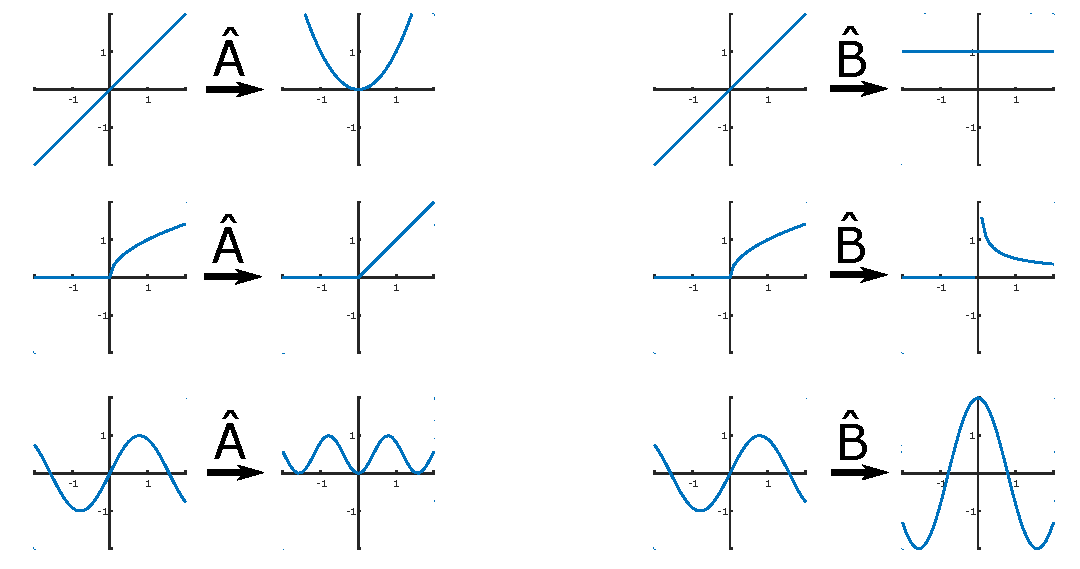
\includegraphics[width=\textwidth]{includes/operators-FIGURES/functions_operators}}
			\vspace{0.2in}
		
			\begin{parts}
			
				\part Describe, in words, what each operator does to a function.
				
					\begin{solution}[2.3in]
					\end{solution}
				
				\part Fill in the blanks by writing mathematical forms for each operator:
				
					\begin{align*}
						\hat A f(x) =  \raisebox{-2ex}{\framebox(60,30){}} & & \hat B f(x) =  \raisebox{-2ex}{\framebox(60,30){}}				
					\end{align*}
				
				\contdnewpg
				\part Predict what functions would result from the following operations:
				
		\vspace{0.2in}	\centerline{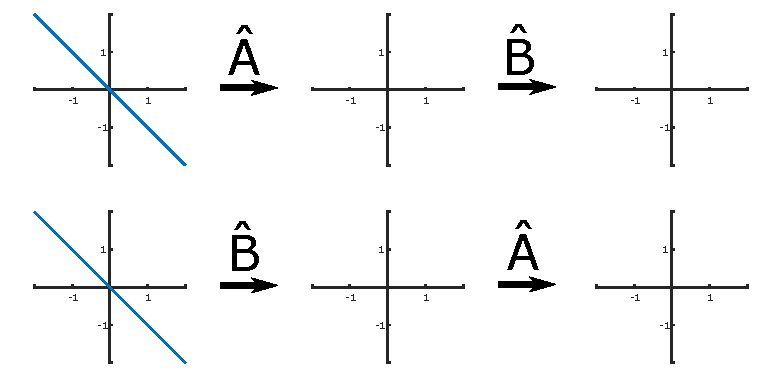
\includegraphics[width=0.7\textwidth]{includes/operators-FIGURES/functions_commutation.pdf}}
			
				\vspace{0.2in}
				
				If the function on the left is $f(x)$, then one of the plots on the right corresponds to $\hat A \hat B f(x)$ and one corresponds to $\hat B \hat A f(x)$.  Circle the plot that you think corresponds to $\hat A \hat B f(x)$.
				
					\vspace{0.2in}
				
				\part From your results, do you think $\hat A \hat B \ket{\Psi}$ will usually be equal to $\hat B \hat A  \ket{\Psi}$?  Why or why not?
				
					\begin{solution}[2in]
					\end{solution}
				
				\part Are there any functions $f(x)$ and $g(x)$ for which $\hat A f(x) = f(x)$ and $\hat B g(x) = g(x)$?  If so, what are they?
				
					\begin{solution}[2.25in]
					\end{solution}
			\end{parts}	
	
	\end{questions}

	\stophere